\documentclass[]{standalone}
\setbeamertemplate{itemize item}[circle]

\begin{document}
	\begin{frame}{Sickle Cell Disease and Silent Cerebral Infarcts}{}
	\begin{itemize}
		\item Sickle Cell Disease (SCD) is a group of inherited red blood cell disorders that causes abnormal hemoglobin.
		
		\item Silent Cerebral Infarcts (SCIs) are defined as abnormal MRI of the brain in the setting of a normal neurologic examination.
	\end{itemize}
	\begin{columns}
		\begin{column}{0.45\textwidth}
		SCIs appear as:
			\begin{itemize}
			\item \textbf{Hypointense} regions in T1W images.
			\item \textbf{Hyperintense} regions in T2W and FLAIR images.
			\end{itemize}
			
		\end{column}
		
		\begin{column}{0.55\textwidth}
			\begin{figure}[h!]
				\begin{subfigure}[b]{0.25\textwidth}
					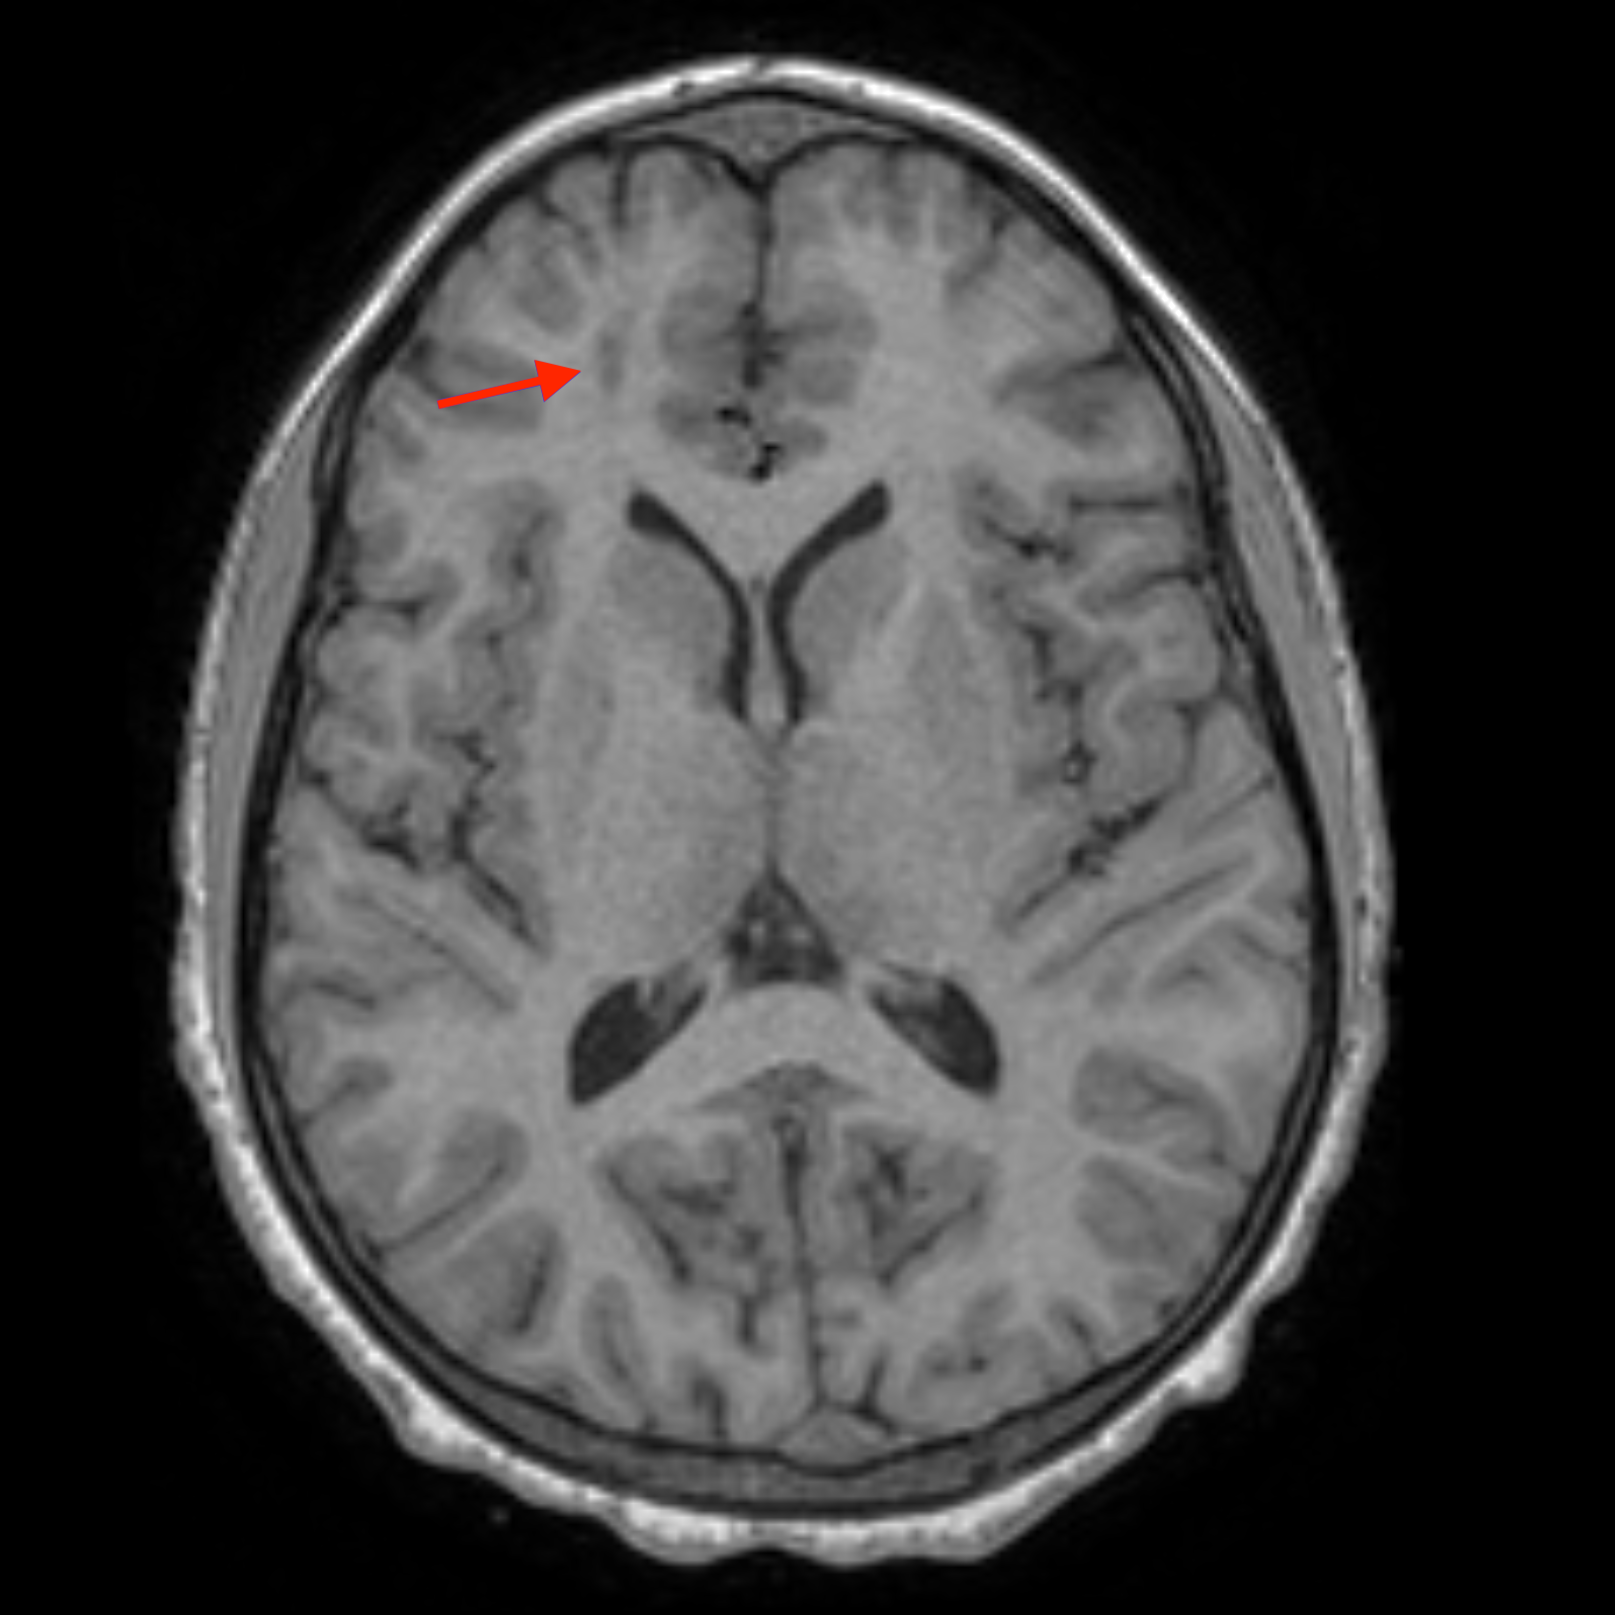
\includegraphics[scale=0.055]{./IMG/Lesion_T1.png}
				\end{subfigure}
				\hspace{32pt}
				\begin{subfigure}[b]{0.25\textwidth}
					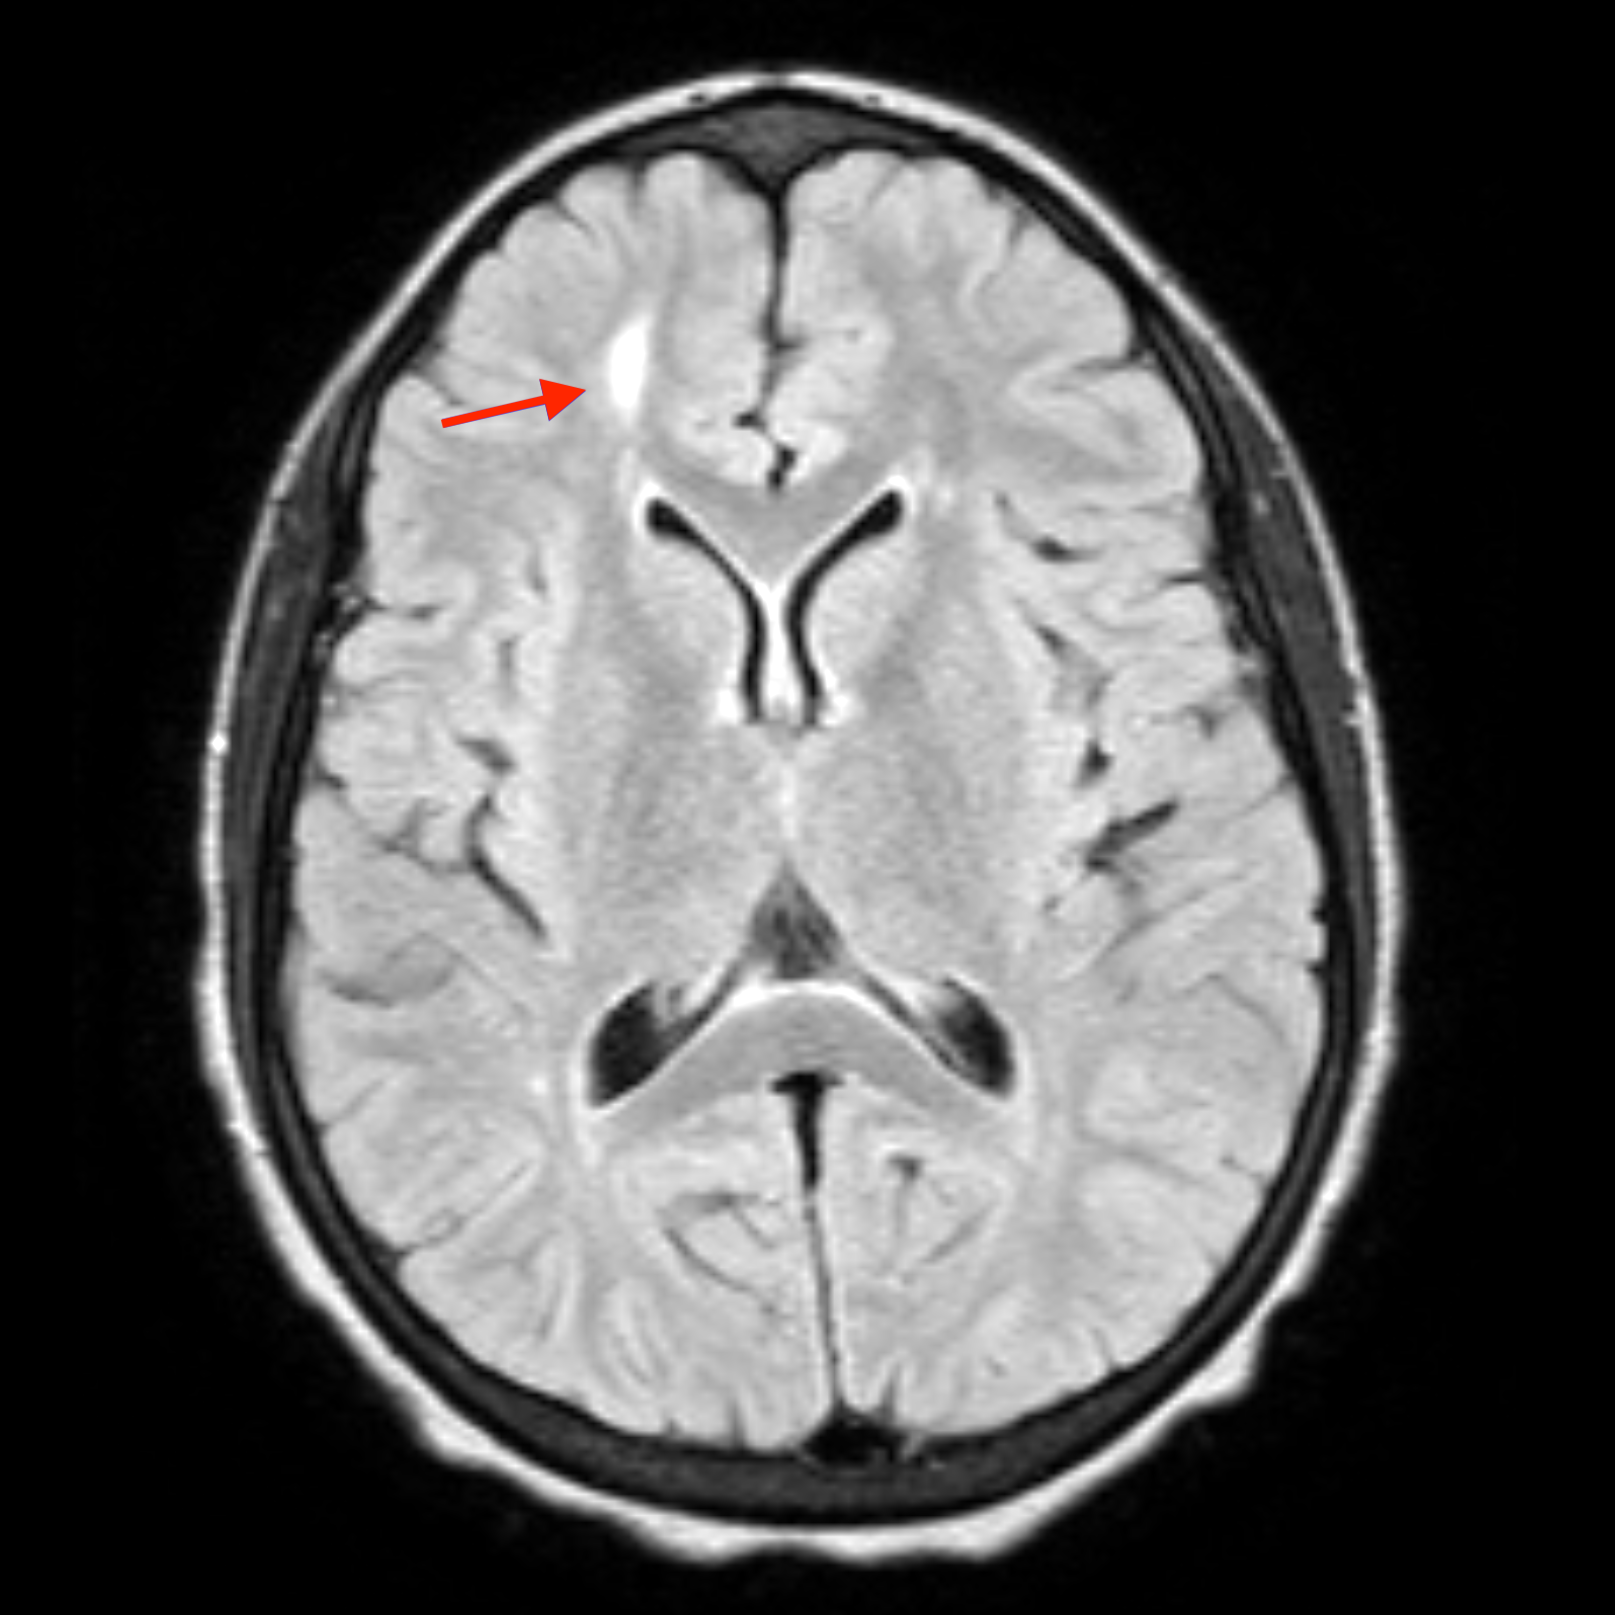
\includegraphics[scale=0.055]{./IMG/Lesion_flair.png}
				\end{subfigure}
				\hspace{20pt}
			\end{figure}
		\end{column}
	\end{columns}
	\end{frame}
\end{document}
